\chapter{Supplementary material for analysis}
\clearpage
\section{Quark-gluon discriminator study}

The $p_{t}D$ in terms of jet $\eta$ in different jet flavors is shown in Fig~\ref{fig:c4ttqgptdjeteta}.
\begin{figure}[htbp]
 \begin{center}
  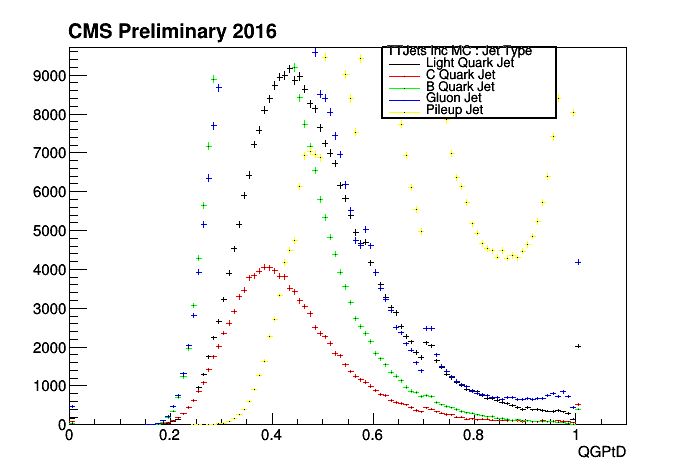
\includegraphics[width=0.45\textwidth]{sections/mc4/TopTagger/figures/_b_qgptdjetetabin0_.png}
  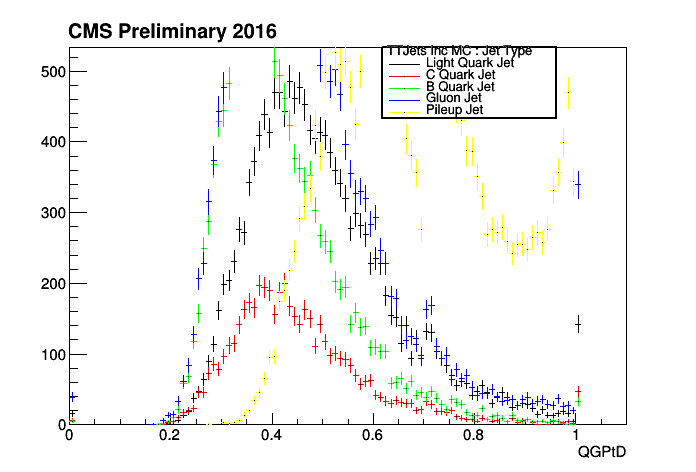
\includegraphics[width=0.45\textwidth]{sections/mc4/TopTagger/figures/_b_qgptdjetetabin1_.png} \\
  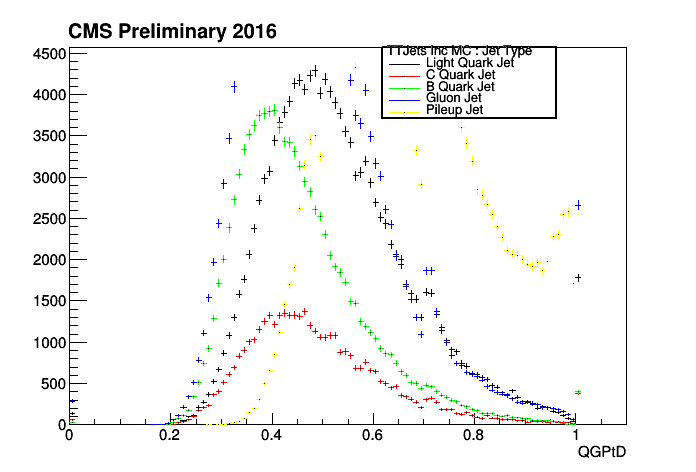
\includegraphics[width=0.45\textwidth]{sections/mc4/TopTagger/figures/_b_qgptdjetetabin2_.png}
  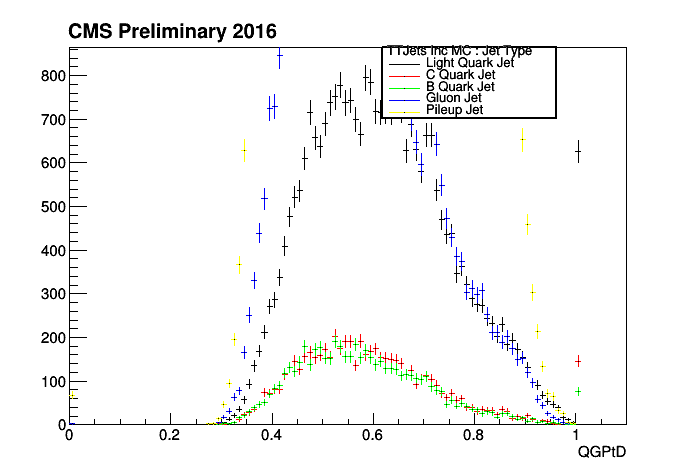
\includegraphics[width=0.45\textwidth]{sections/mc4/TopTagger/figures/_b_qgptdjetetabin3_.png} \\
  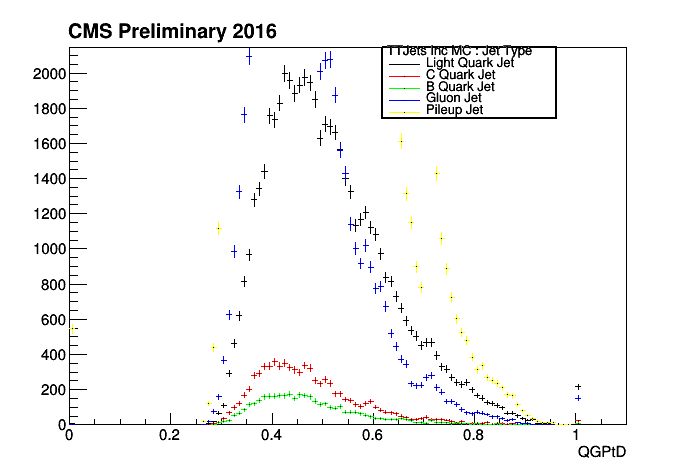
\includegraphics[width=0.45\textwidth]{sections/mc4/TopTagger/figures/_b_qgptdjetetabin4_.png}
  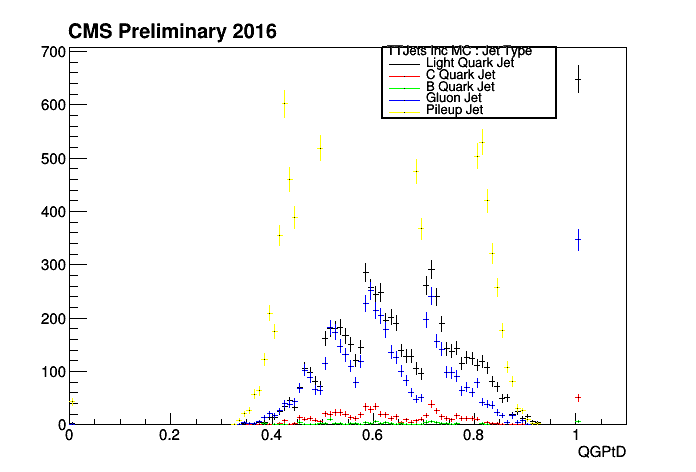
\includegraphics[width=0.45\textwidth]{sections/mc4/TopTagger/figures/_b_qgptdjetetabin5_.png}
 \end{center}
 \caption{Top left: Quark Gluon $p_{t}D$ for jet $\eta$ bin 1; Top right: jet $\eta$ bin 2; Middle left: jet $\eta$ bin 3; Middle right: jet $\eta$ bin 4; Middle left: jet $\eta$ bin 5; Middle right: jet $\eta$ bin 6}
 \label{fig:c4ttqgptdjeteta}
\end{figure}

The $p_{t}D$ in terms of jet $p_{T}$ in different jet flavors is shown in Fig~\ref{fig:c4ttqgptdjetpt}.
\begin{figure}[htbp]
 \begin{center}
  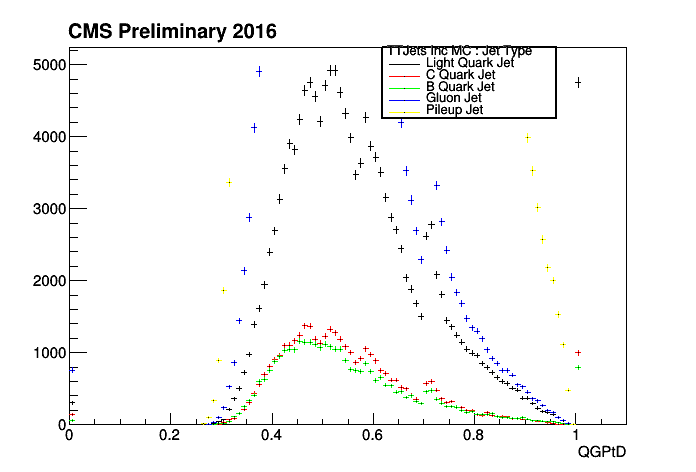
\includegraphics[width=0.45\textwidth]{sections/mc4/TopTagger/figures/_b_qgptdjetptbin0_.png}
  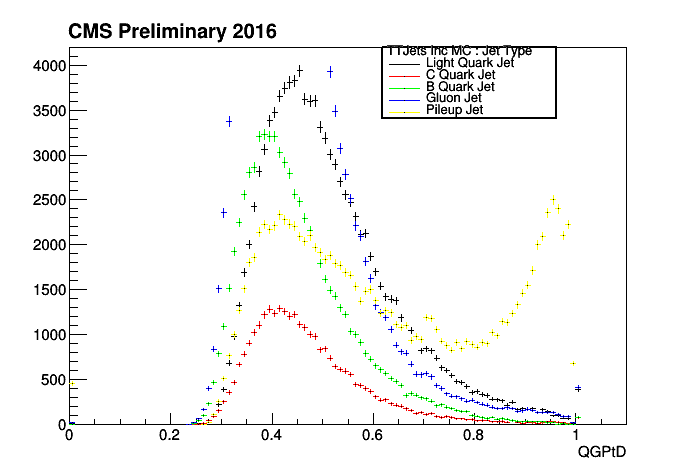
\includegraphics[width=0.45\textwidth]{sections/mc4/TopTagger/figures/_b_qgptdjetptbin1_.png} \\
  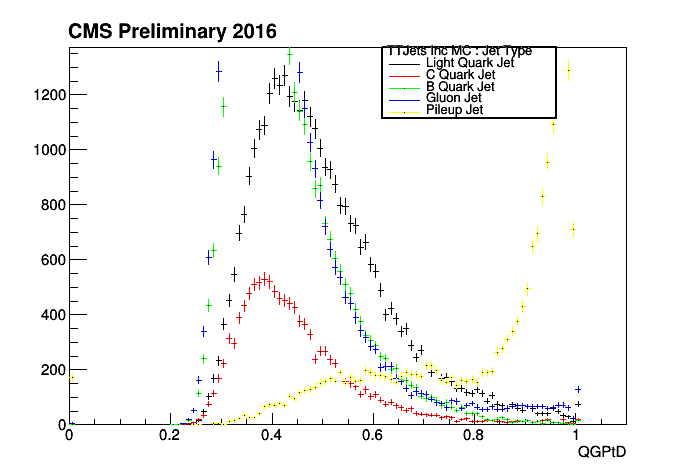
\includegraphics[width=0.45\textwidth]{sections/mc4/TopTagger/figures/_b_qgptdjetptbin2_.png}
  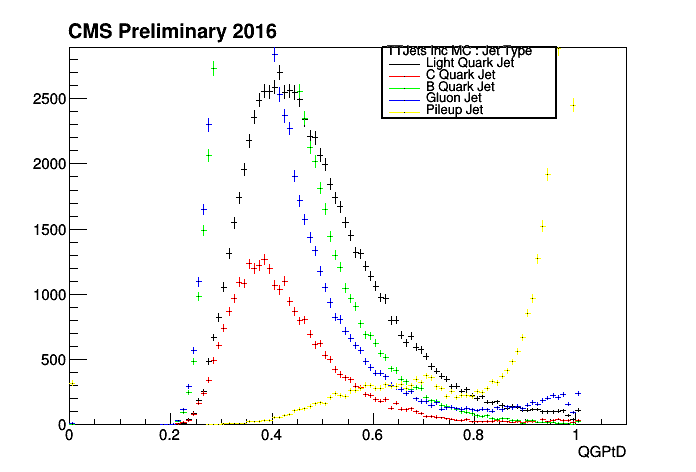
\includegraphics[width=0.45\textwidth]{sections/mc4/TopTagger/figures/_b_qgptdjetptbin3_.png} \\
  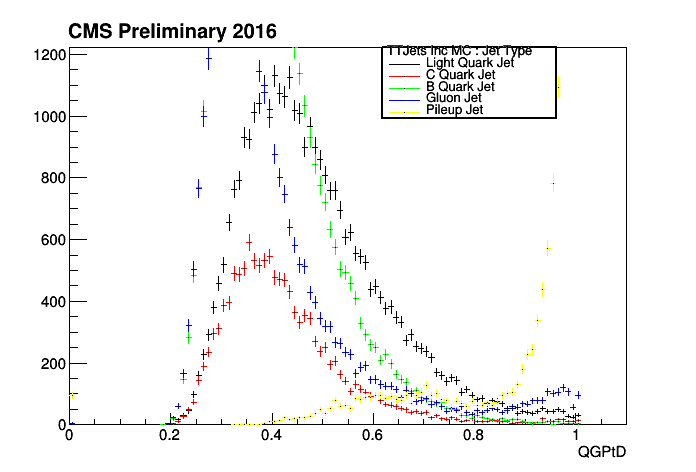
\includegraphics[width=0.45\textwidth]{sections/mc4/TopTagger/figures/_b_qgptdjetptbin4_.png}
  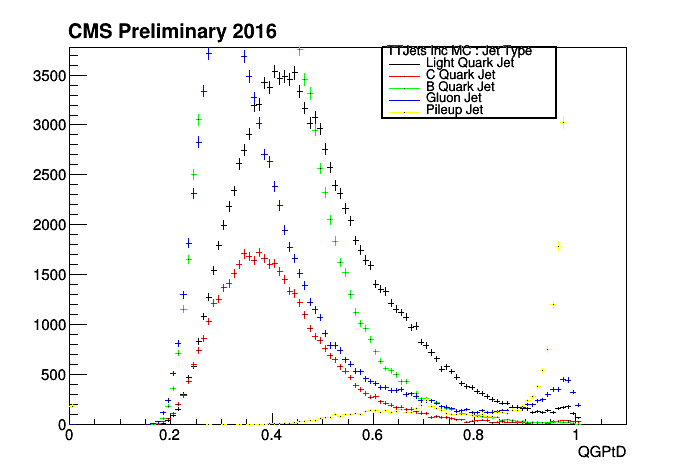
\includegraphics[width=0.45\textwidth]{sections/mc4/TopTagger/figures/_b_qgptdjetptbin5_.png}
 \end{center}
 \caption{Top left: Quark Gluon $p_{t}D$ for jet $p_{T}$ bin 1; Top right: jet $p_{T}$ bin 2; Middle left: jet $p_{T}$ bin 3; Middle right: jet $p_{T}$ bin 4; Middle left: jet $p_{T}$ bin 5; Middle right: jet $p_{T}$ bin 6}
 \label{fig:c4ttqgptdjetpt}
\end{figure}

The multiplicity in terms of jet $\eta$ in different jet flavors is shown in Fig~\ref{fig:c4ttqgmultjeteta}.
\begin{figure}[htbp]
 \begin{center}
  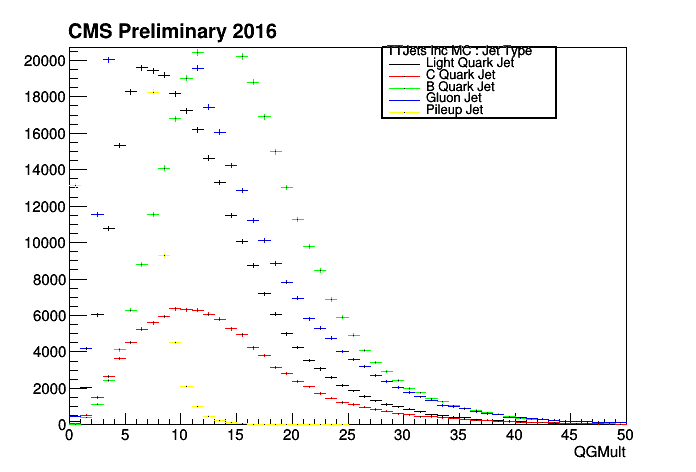
\includegraphics[width=0.45\textwidth]{sections/mc4/TopTagger/figures/_b_qgmultjetetabin0_.png}
  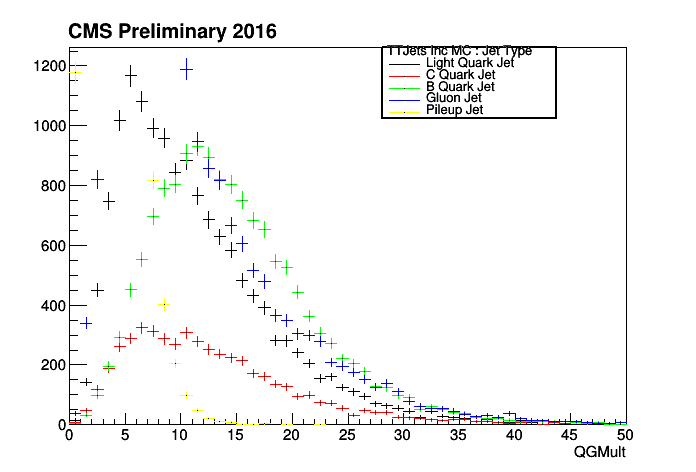
\includegraphics[width=0.45\textwidth]{sections/mc4/TopTagger/figures/_b_qgmultjetetabin1_.png} \\
  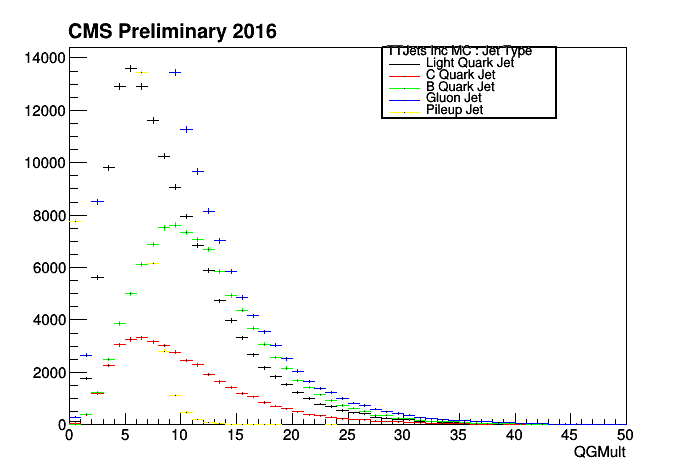
\includegraphics[width=0.45\textwidth]{sections/mc4/TopTagger/figures/_b_qgmultjetetabin2_.png}
  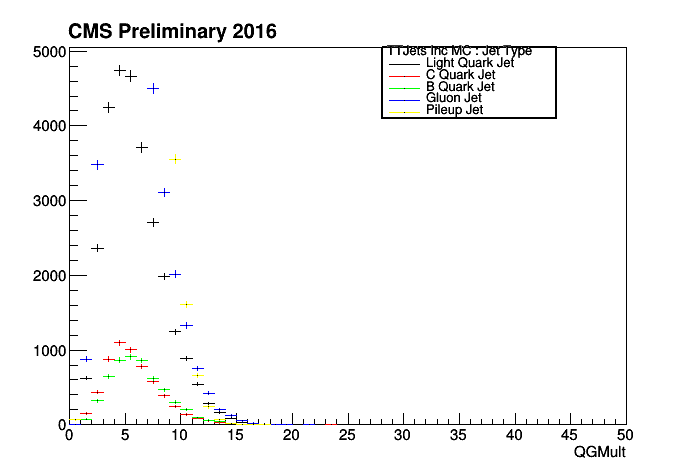
\includegraphics[width=0.45\textwidth]{sections/mc4/TopTagger/figures/_b_qgmultjetetabin3_.png} \\
  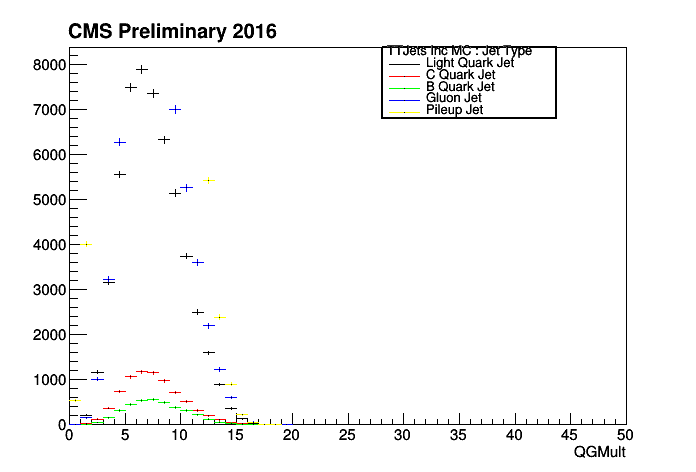
\includegraphics[width=0.45\textwidth]{sections/mc4/TopTagger/figures/_b_qgmultjetetabin4_.png}
  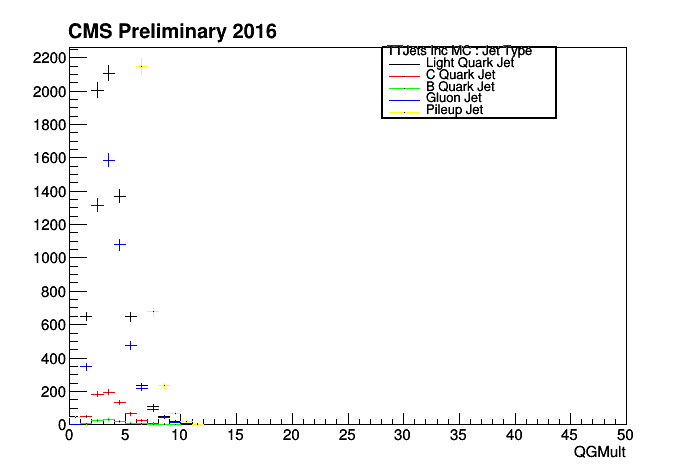
\includegraphics[width=0.45\textwidth]{sections/mc4/TopTagger/figures/_b_qgmultjetetabin5_.png}
 \end{center}
 \caption{Top left: Quark Gluon multiplicity for jet $\eta$ bin 1; Top right: jet $\eta$ bin 2; Middle left: jet $\eta$ bin 3; Middle right: jet $\eta$ bin 4; Middle left: jet $\eta$ bin 5; Middle right: jet $\eta$ bin 6}
 \label{fig:c4ttqgmultjeteta}
\end{figure}

The multiplicity in terms of jet $p_{T}$ in different jet flavors is shown in Fig~\ref{fig:c4ttqgmultjetpt}.
\begin{figure}[htbp]
 \begin{center}
  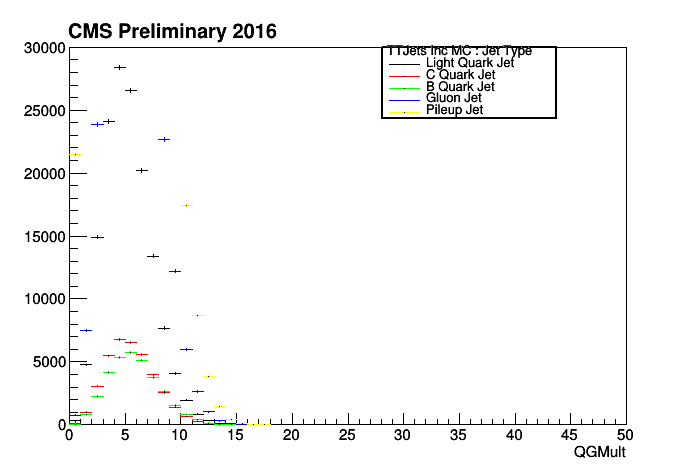
\includegraphics[width=0.45\textwidth]{sections/mc4/TopTagger/figures/_b_qgmultjetptbin0_.png}
  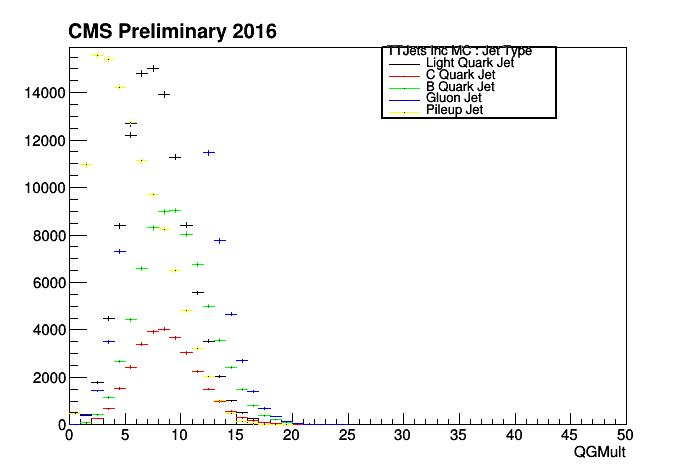
\includegraphics[width=0.45\textwidth]{sections/mc4/TopTagger/figures/_b_qgmultjetptbin1_.png} \\
  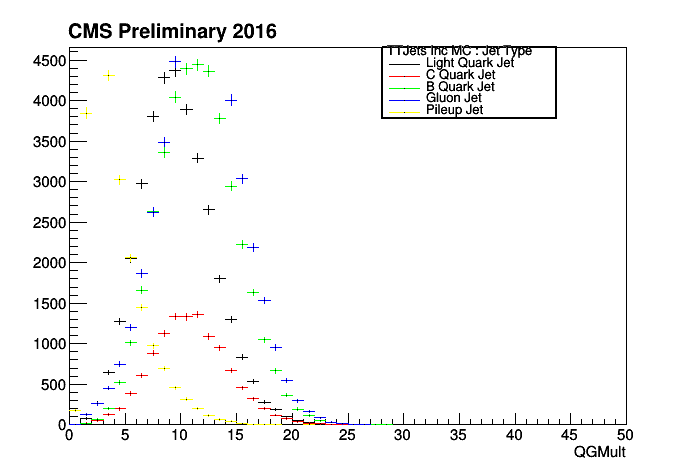
\includegraphics[width=0.45\textwidth]{sections/mc4/TopTagger/figures/_b_qgmultjetptbin2_.png}
  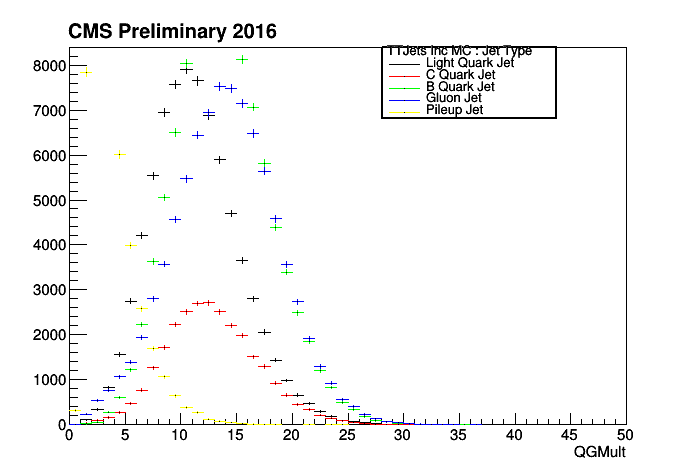
\includegraphics[width=0.45\textwidth]{sections/mc4/TopTagger/figures/_b_qgmultjetptbin3_.png} \\
  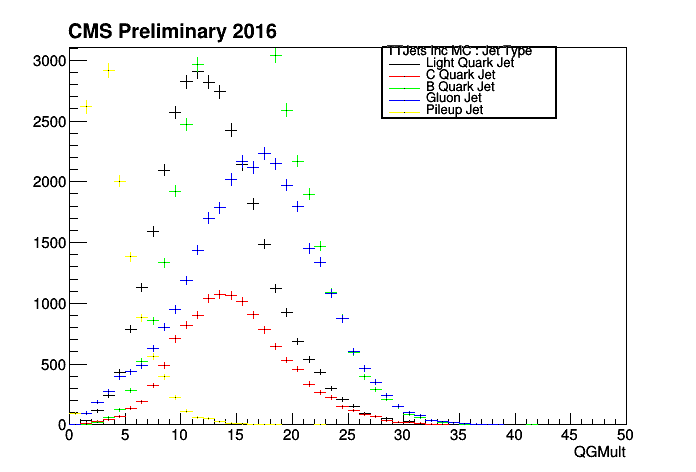
\includegraphics[width=0.45\textwidth]{sections/mc4/TopTagger/figures/_b_qgmultjetptbin4_.png}
  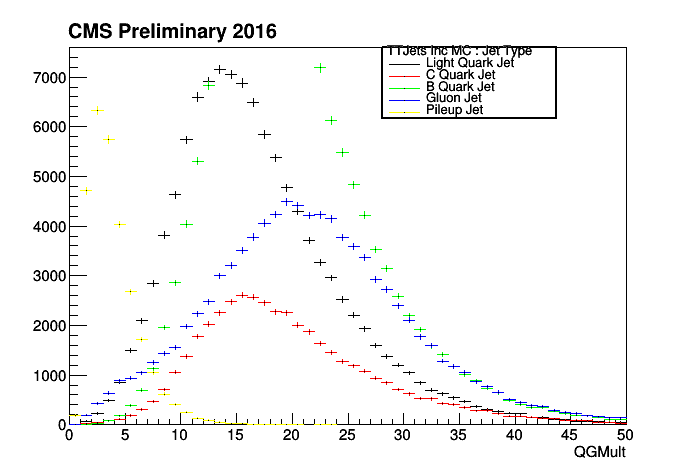
\includegraphics[width=0.45\textwidth]{sections/mc4/TopTagger/figures/_b_qgmultjetptbin5_.png}
 \end{center}
 \caption{Top left: Quark Gluon multiplicity for jet $p_{T}$ bin 1; Top right: jet $p_{T}$ bin 2; Middle left: jet $p_{T}$ bin 3; Middle right: jet $p_{T}$ bin 4; Middle left: jet $p_{T}$ bin 5; Middle right: jet $p_{T}$ bin 6}
 \label{fig:c4ttqgmultjetpt}
\end{figure}

The Axis2 in terms of jet $\eta$ in different jet flavors is shown in Fig~\ref{fig:c4ttqgaxis2jeteta}.
\begin{figure}[htbp]
 \begin{center}
  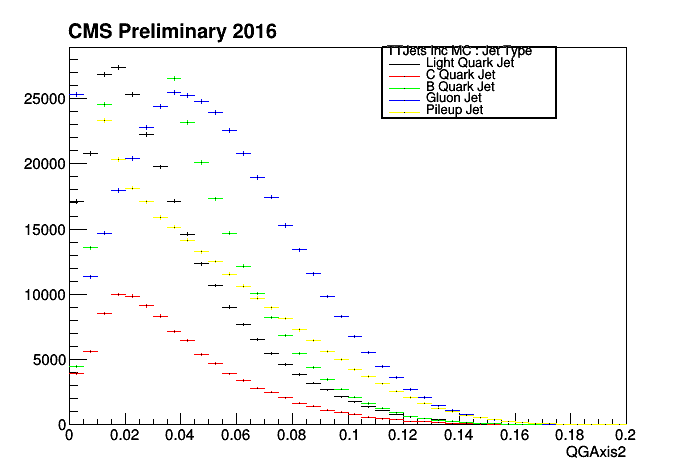
\includegraphics[width=0.45\textwidth]{sections/mc4/TopTagger/figures/_b_qgaxis2jetetabin0_.png}
  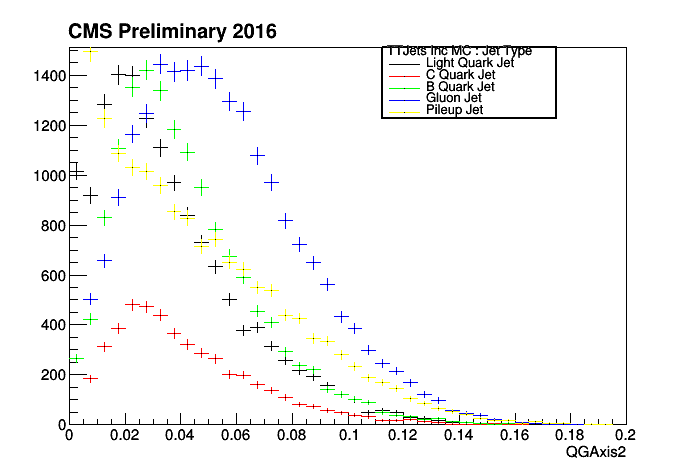
\includegraphics[width=0.45\textwidth]{sections/mc4/TopTagger/figures/_b_qgaxis2jetetabin1_.png} \\
  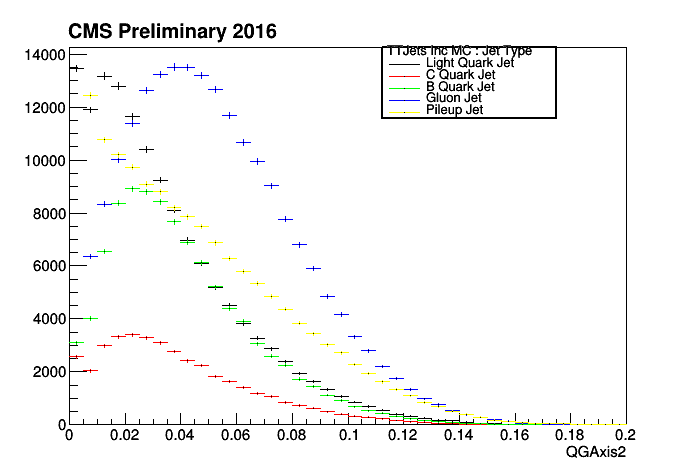
\includegraphics[width=0.45\textwidth]{sections/mc4/TopTagger/figures/_b_qgaxis2jetetabin2_.png}
  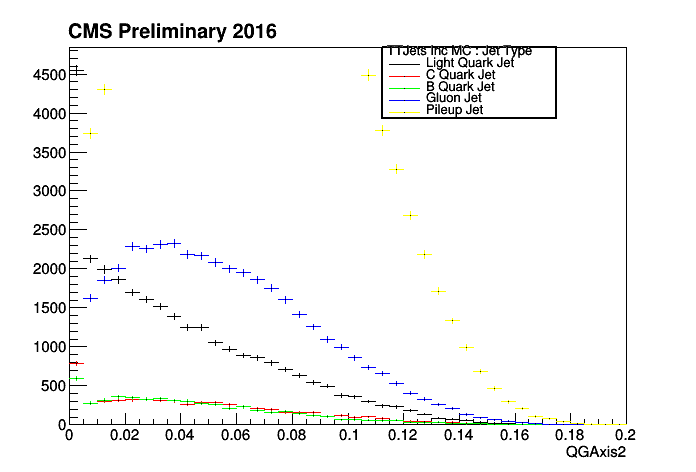
\includegraphics[width=0.45\textwidth]{sections/mc4/TopTagger/figures/_b_qgaxis2jetetabin3_.png} \\
  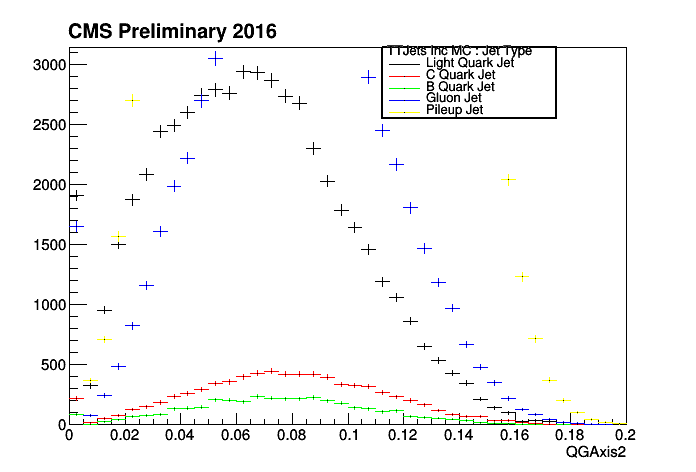
\includegraphics[width=0.45\textwidth]{sections/mc4/TopTagger/figures/_b_qgaxis2jetetabin4_.png}
  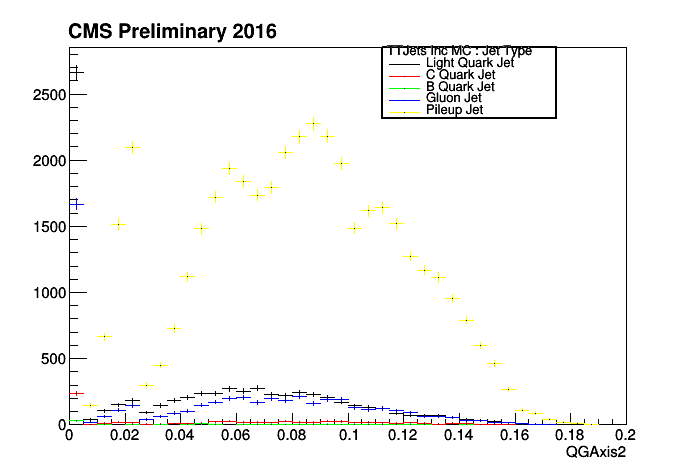
\includegraphics[width=0.45\textwidth]{sections/mc4/TopTagger/figures/_b_qgaxis2jetetabin5_.png}
 \end{center}
 \caption{Top left: Quark Gluon Axis2 for jet $\eta$ bin 1; Top right: jet $\eta$ bin 2; Middle left: jet $\eta$ bin 3; Middle right: jet $\eta$ bin 4; Middle left: jet $\eta$ bin 5; Middle right: jet $\eta$ bin 6}
 \label{fig:c4ttqgaxis2jeteta}
\end{figure}

The Axis2 in terms of jet $p_{T}$ in different jet flavors is shown in Fig~\ref{fig:c4ttqgaxis2jetpt}.
\begin{figure}[htbp]
 \begin{center}
  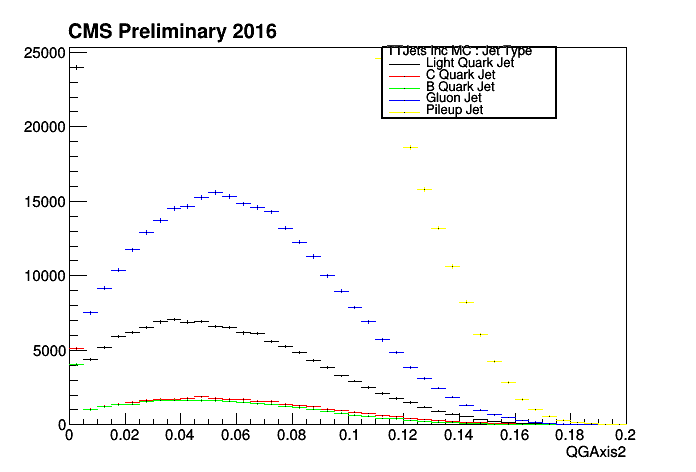
\includegraphics[width=0.45\textwidth]{sections/mc4/TopTagger/figures/_b_qgaxis2jetptbin0_.png}
  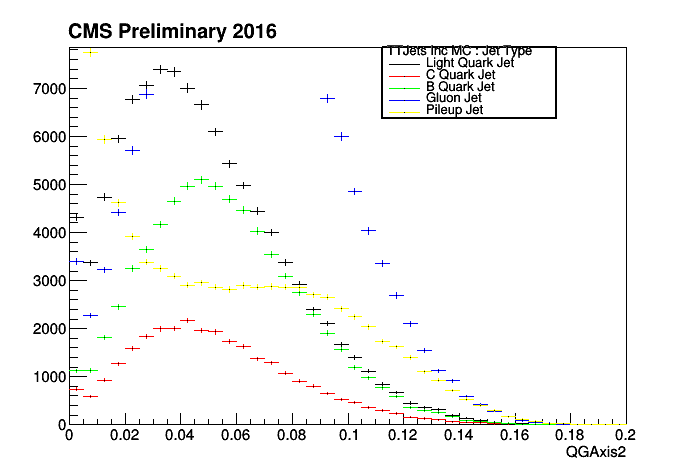
\includegraphics[width=0.45\textwidth]{sections/mc4/TopTagger/figures/_b_qgaxis2jetptbin1_.png} \\
  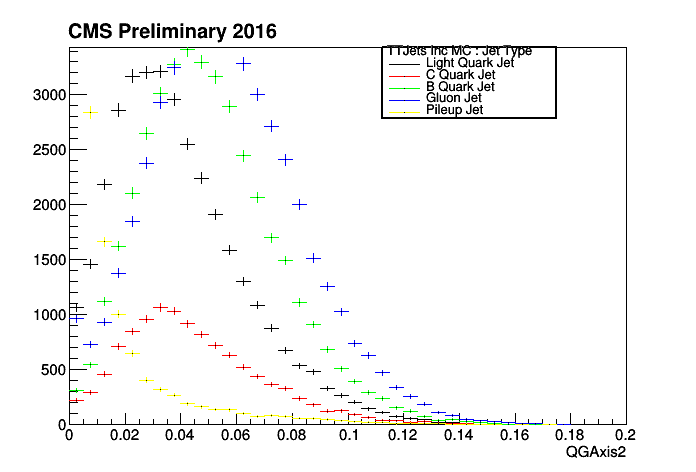
\includegraphics[width=0.45\textwidth]{sections/mc4/TopTagger/figures/_b_qgaxis2jetptbin2_.png}
  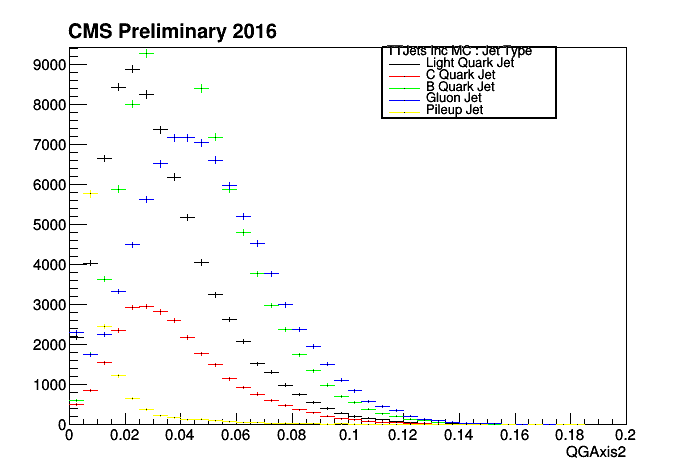
\includegraphics[width=0.45\textwidth]{sections/mc4/TopTagger/figures/_b_qgaxis2jetptbin3_.png} \\
  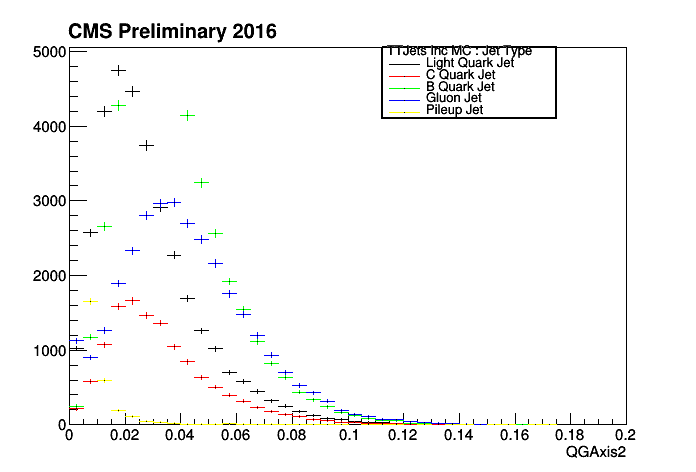
\includegraphics[width=0.45\textwidth]{sections/mc4/TopTagger/figures/_b_qgaxis2jetptbin4_.png}
  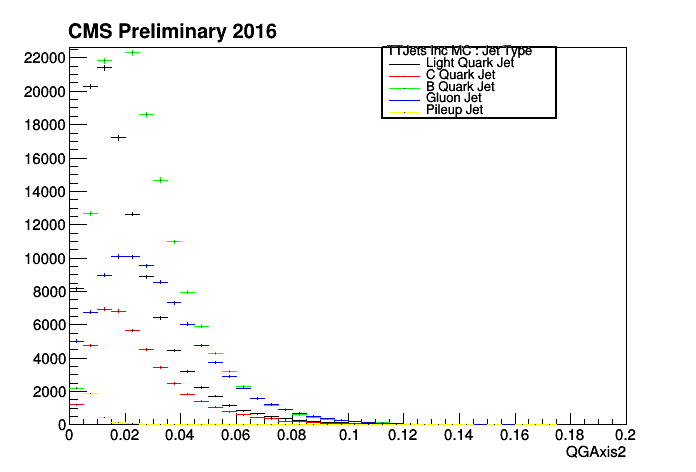
\includegraphics[width=0.45\textwidth]{sections/mc4/TopTagger/figures/_b_qgaxis2jetptbin5_.png}
 \end{center}
 \caption{Top left: Quark Gluon Axis2 for jet $p_{T}$ bin 1; Top right: jet $p_{T}$ bin 2; Middle left: jet $p_{T}$ bin 3; Middle right: jet $p_{T}$ bin 4; Middle left: jet $p_{T}$ bin 5; Middle right: jet $p_{T}$ bin 6}
 \label{fig:c4ttqgaxis2jetpt}
\end{figure}

\clearpage
\section{Di-Top jets event display}
The Event with two reconstructed top jets are demonstrated in Fig~\ref{fig:appttevtdisplay}. The jet energies and \MET shown are without energy correction.
\begin{figure}[htbp]
 \begin{center}
  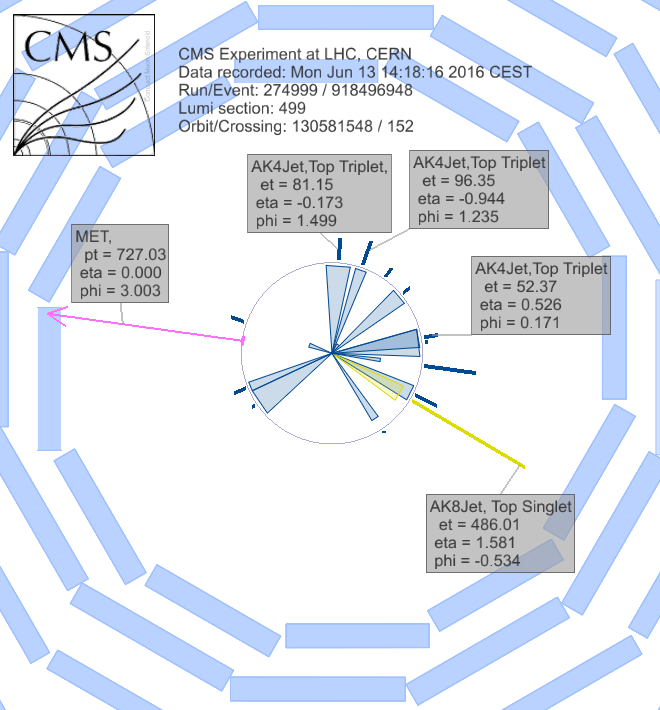
\includegraphics[width=0.45\textwidth]{figures/appendix/appendix_tagger_Run2016B_2t_1j3j-274999_918496948_499_RhoPhi.png}
  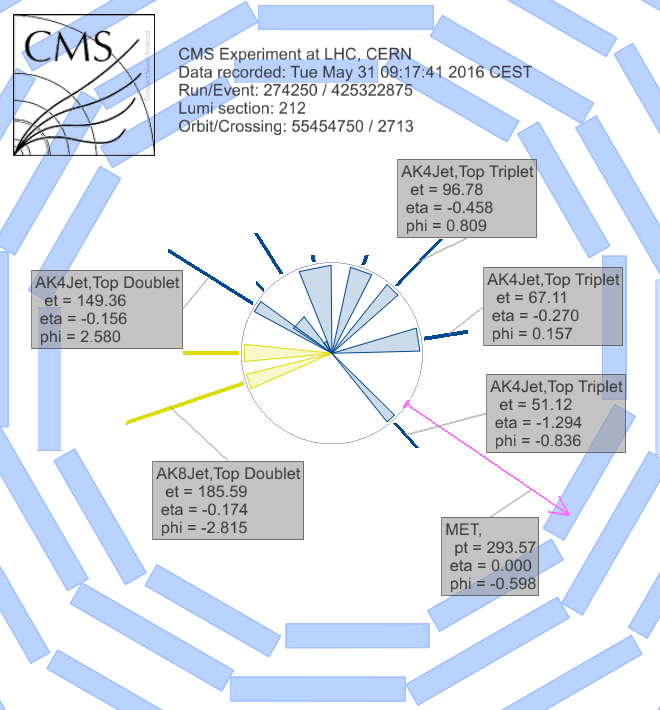
\includegraphics[width=0.45\textwidth]{figures/appendix/appendix_tagger_Run2016B_2t_2j3j-274250_425322875_212_RhoPhi.png}
\end{center} \caption{Event display for di-topjets event in data. Left plot is one mono-jet top and one triple-jet top, Right plot is one di-jet top and one triple-jet top. Yellow line is fat jet (anti-$k_{T}$ R=0.8), blue line is normal jet (anti-$k_{T}$ R=0.4), the purple line is \MET.}
 \label{fig:appttevtdisplay}
\end{figure}

\clearpage
\section{Simplified top tagger, aggregate search bin and results}

Simplified top tagger and 10 aggregate search bins are defined to simplify the use of our data. We drop the quark gluon discriminator, therefore theorist can repeat our tagging algorithm. As given in Table~\ref{tab:aggBinDescrption}, the aggregate search bins are not exclusive. The first four aggregate regions represent topologies of general interest. The fifth and sixth are sensitive to direct top squark pair production. The seventh region targets the large $\Delta M(\gluino,\chiOneZero)$ region of T5ttcc-like models, while the final three target events with a large number of top quarks such as are produced in the T1tttt and T5tttt models.

\begin{table}[htb]
\centering
  \caption{Definition of the aggregate search regions.}
\label{tab:aggBinDescrption}
\renewcommand{\arraystretch}{1.15}
\begin{tabular}{cccccc}
\hline
Region & \ntops & \nbjets & \MTTwo [GeV] & \MET [GeV] & Motivation \\
\hline
1  & $\geq1$     & $\geq1$      & $\geq200$       & $\geq250$        & \specialcell{Events satisfying \\ selection criteria}      \\
\hline
2  & $\geq2$     & $\geq2$      & $\geq200$       & $\geq250$        & \specialcell{Events with \\ $\ntops \ge 2$ and $\nbjets \ge 2$}  \\
\hline
3  & $\geq3$     & $\geq1$      & $\geq200$       & $\geq250$        & \specialcell{Events with \\ $\ntops \ge 3$ and $\nbjets \ge 1$}  \\
\hline
4  & $\geq3$     & $\geq3$      & $\geq200$       & $\geq250$        & \specialcell{T5tttt; small $\Delta M(\gluino,\chiOneZero)$ \\ and $m_{\chiOneZero}<m_{t}$}     \\
\hline
5  & $\geq2$     & $\geq1$      & $\geq200$       & $\geq400$        & \specialcell{T2tt; \\ small $\Delta M(\sTop,\chiOneZero)$}      \\
\hline
6  & $\geq1$     & $\geq2$      & $\geq600$       & $\geq400$        & \specialcell{T2tt; \\ large $\Delta M(\sTop,\chiOneZero)$}      \\
\hline
Region & \ntops & \nbjets & \HT [GeV] & \MET [GeV] & Motivation \\
\hline
7  & $\geq1$     & $\geq2$      & $\geq1400$      & $\geq500$        & \specialcell{T1ttbb and T5ttcc; \\ large $\Delta M(\gluino,\chiOneZero)$}    \\
\hline
8  & $\geq2$     & $\geq3$      & $\geq600$       & $\geq350$        & \specialcell{T1tttt; \\ small $\Delta M(\gluino,\chiOneZero)$}    \\
\hline
9  & $\geq2$     & $\geq3$      & $\geq300$       & $\geq500$        & \specialcell{T1/T5tttt and T1ttbb; \\ intermediate $\Delta M(\gluino,\chiOneZero)$}    \\
\hline
10 & $\geq2$     & $\geq3$      & $\geq1300$      & $\geq500$        & \specialcell{T1/T5tttt; \\ large $\Delta M(\gluino,\chiOneZero)$}    \\
\hline
\end{tabular}
\end{table}

The aggregate search bin results are shown in Fig~\ref{fig:aggSearchBinResults} and Table~\ref{tab:agg_sb_obs_pred}, using the same background estimation methods described in this thesis.

\begin{figure}[htb]
  \begin{center}
  \begin{tabular}{cc}
  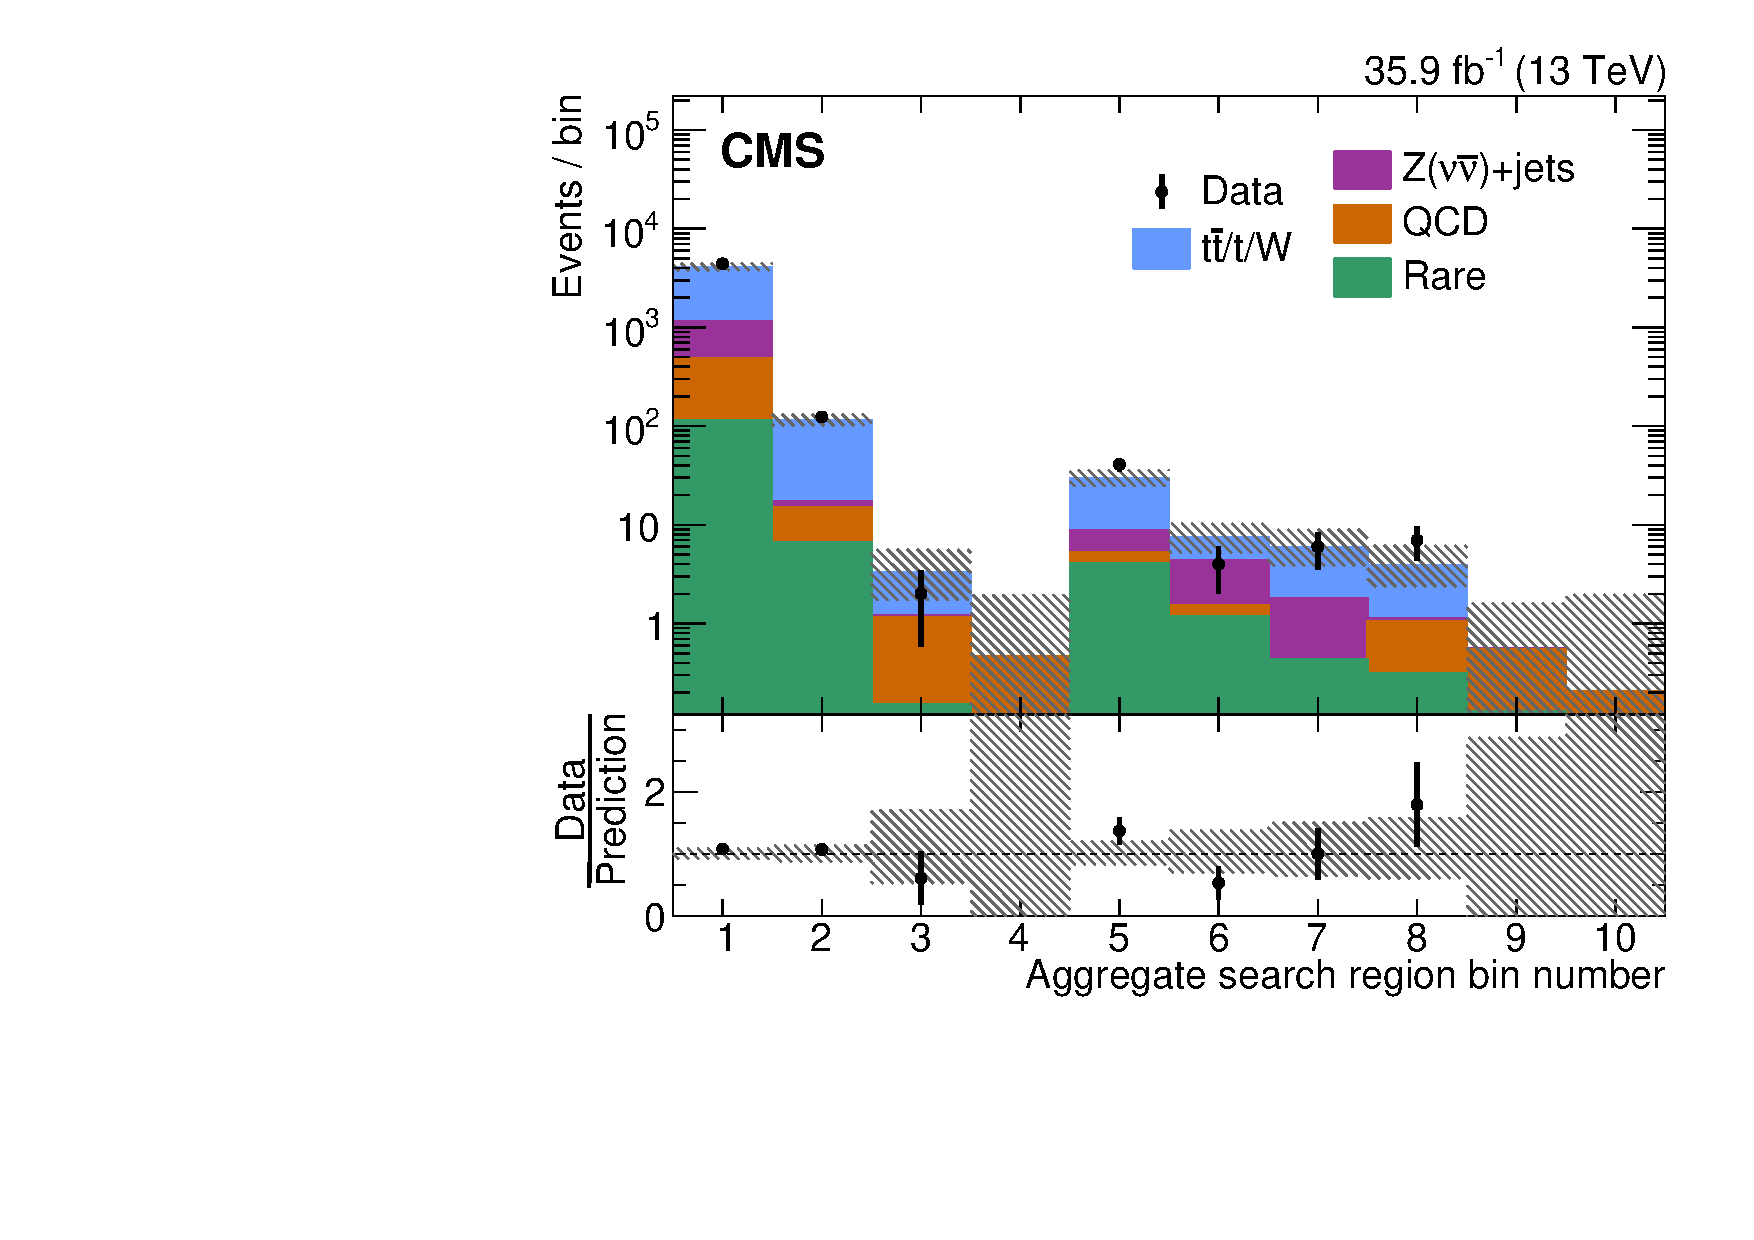
\includegraphics[angle=0,width=0.9\textwidth]{figures/appendix/aggregatedSearchBins.pdf}
  \end{tabular}
  \caption{
  Observed event yields (black points)
  and predicted SM background (filled solid areas)
  for the 10 aggregate search regions.
  The lower panel shows the ratio of the data to
  the total background prediction.
  The hatched bands correspond to the total uncertainty in the
  background prediction.
   }
    \label{fig:aggSearchBinResults}
  \end{center}
\end{figure}

\begin{table}[htb]
\centering
\caption{
The observed number of events and the total background prediction
for the aggregate search regions.
The first uncertainty in the background prediction is
statistical and the second is systematic.
}
\label{tab:agg_sb_obs_pred}
\renewcommand{\arraystretch}{1.30}
 \begin{tabular}{cccccccccccc}
  \hline
     Search region &  \ntops &    \nbjets &   \MTTwo [GeV] &     \MET [GeV]  & Data & Predicted background \\
  \hline
    1 &  $\geq 1$ &   $\geq 1$ &   $\geq 200$ &   $\geq 250$  &  4424 &   $4100\pm 50^{ +390}_{ -340}$ \\
    2 &  $\geq 2$ &   $\geq 2$ &   $\geq 200$ &   $\geq 250$  &   124 &   $116\pm 8^{  +15} _{  -12}$ \\
    3 &  $\geq 3$ &   $\geq 3$ &   $\geq 200$ &   $\geq 250$  &     0 &   $0.5^{ +1.4} _{ -0.4}\pm 0.5$ \\
    4 &  $\geq 3$ &   $\geq 1$ &   $\geq 200$ &   $\geq 250$  &     2 &   $3.3^{ +2.0} _{ -1.1}$ $^{ +1.2} _{ -1.1}$ \\
    5 &  $\geq 2$ &   $\geq 1$ &   $\geq 200$ &   $\geq 400$  &    41 &   $30^{   +4} _{   -3}$ $^{   +5} _{   -4}$ \\
    6 &  $\geq 1$ &   $\geq 2$ &   $\geq 600$ &   $\geq 400$  &     4 &   $7.5^{ +2.1} _{ -1.2}$ $^{ +2.0} _{ -1.9}$ \\
  \hline
     Search region &  \ntops &    \nbjets &   \HT [GeV] &     \MET [GeV]  &  Data & Predicted background \\
  \hline
    7 &  $\geq 1$ &   $\geq 2$ &   $\geq 1400$ &  $\geq 500$  &     6 &   $6.0^{ +2.7} _{ -1.5}\pm 1.5$ \\
    8 &  $\geq 2$ &   $\geq 3$ &   $\geq 600$  &  $\geq 350$  &     7 &   $3.9^{ +2.1} _{ -1.2}\pm 0.9$ \\
    9 &  $\geq 2$ &   $\geq 3$ &   $\geq 300$  &  $\geq 500$  &     0 &   $0.6^{ +1.0} _{ -0.4}\pm 0.4$ \\
   10 &  $\geq 2$ &   $\geq 3$ &   $\geq 1300$ &  $\geq 500$  &     0 &   $0.2^{ +1.8} _{ -0.3}\pm 0.2$ \\
  \hline
 \end{tabular}
\end{table}
